\begin{multicols}{2}
\textbf{Ingredients}
\begin{itemize}
\item 1 lb linguine\quad
\item 2 lbs peeled \& deveined shrimp
\item 3-4 shallots
\item 1 cup dry white wine (I use Pinot Grigio)
\item 4 tbsp butter
\item 4 tbsp. olive oil
\item $\sim 5$ cloves of garlic (minced)
\item The juice of 2 lemons
\item 2 tbsp. red pepper flakes
\item 2 tsp. salt
\item 1 tsp. black pepper
\item $\frac{1}{4}$ cup chopped parsley 



\end{itemize}


\columnbreak
\textbf{Procedure:}
\medskip


\begin{enumerate}
\item Begin by boiling water in a large pot for the pasta. When it has come to a boil, add a couple of teaspoons of salt and add linguine. Stir to make sure the pasta separates. Cover. When water returns to a boil, cook for 7-9 minutes. Drain pasta. 


\medskip
\item Meanwhile, in a large skillet, melt 2 tbsp of olive oil in 2 tbsp butter over medium-high heat. Saute the shallots, garlic, and red pepper flakes until the shallots are translucent ($\sim$4 minutes). Season the shrimp with salt and pepper; add them to the pan and cook until they have turned pink. Remove shrimp from pan and keep warm. 
\medskip

\item Add wine and lemon juice and bring to a boil. Add 3 tbsp of olive oil and 3 tbsp of butter. When the butter has melted, return the shrimp to the pan along with parsley and cooked pasta. 
\newline 

 \item Stir well and season with salt and pepper. Drizzle olive oil and serve immediately.   

\end{enumerate}
\end{multicols}


\begin{center}
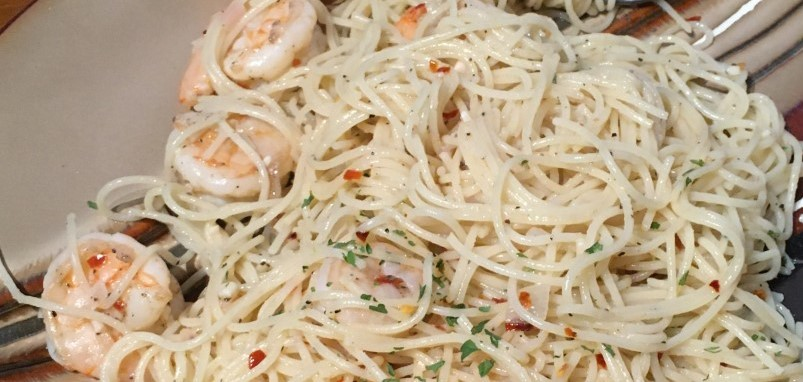
\includegraphics[scale=0.65]{Pasta/Shrimp Scampi/Shrimp Scampi.jpg}
\end{center}
